% Actes EIAH / RJC-EIAH
% S'appuie sur la classe de base llncs,
% avec une gestion de l'utf-8, du français
% Auteurs : Rémi Venant <remi.venant@univ-lemans.fr>
% Version 1.10 - 2023/10/06
%

%%%%%%%%%%%%%%%%%%%%%%%%%%%%%%%%%%%%%%%%%%%%%%%%%%%%%%
%% INCLUSION DES PACKAGES                           %%
%%%%%%%%%%%%%%%%%%%%%%%%%%%%%%%%%%%%%%%%%%%%%%%%%%%%%%
\documentclass[runningheads]{llncs}
\usepackage[utf8]{inputenc} %gestion des fichiers utf8
\PassOptionsToPackage{french}{babel}
\usepackage{babel}
\usepackage[T1]{fontenc}
\usepackage{hyphenat}
\usepackage{subcaption}
\usepackage{graphicx}
\usepackage[dvipsnames]{xcolor}
\usepackage{sectsty}
\usepackage{wrapfig}
\usepackage[titles]{tocloft}
\usepackage{ifthen}
\usepackage{pdfpages}
\usepackage{geometry}
\usepackage[export]{adjustbox}
\usepackage{tocloft}
\usepackage{blindtext}
\usepackage[hidelinks]{hyperref}

%%%%%%%%%%%%%%%%%%%%%%%%%%%%%%%%%%%%%%%%%%%%%%%%%%%%%%
%% DEFINITIONS GENERALES - A APADATER SELON CONF    %%
%%%%%%%%%%%%%%%%%%%%%%%%%%%%%%%%%%%%%%%%%%%%%%%%%%%%%%

% Couleur principale du manuscript (utilisée notamment pour les titres principaux)
\definecolor{ConfColor}{HTML}{AE2573}

% En-têtes des pages paires/impaires (hors articles)
\newcommand{\resetHeadings}{
	\markboth{Catherine Bonnat et Rémi Venant}{Rencontres Jeunes Chercheur·e·s en EIAH 2022, Lille}
}

% Logo de la conférence
\newcommand{\logoConf}[1][0.6]{
	\begin{figure}[h]
		\centering
		\includegraphics[width=#1\textwidth]{Content/figures/logoConf.png}
	\end{figure}
}

%%%%%%%%%%%%%%%%%%%%%%%%%%%%%%%%%%%%%%%%%%%%%%%%%%%%%%%%%%%%%
%% DEFINITION DE COMMANDES (MODIFICATIONS NON REOMMANDEES) %%
%%%%%%%%%%%%%%%%%%%%%%%%%%%%%%%%%%%%%%%%%%%%%%%%%%%%%%%%%%%%%

% Redéfinition de mots usuels
\renewcommand\keywordname{{\bf Mots-cl\'es :}}
\addto\captionsfrench{\renewcommand{\figurename}{\upshape Fig.}}
% Définition du formatage des titres, page blanche
\makeatletter
\renewcommand{\@seccntformat}[1]{}
\makeatother
\sectionfont{\LARGE\centering\color{ConfColor}}
\renewcommand{\contentsname}{Table of contents}
\renewcommand{\cftsecfont}{\normalfont\bfseries\color{ConfColor}}% titles in bold
\renewcommand{\cftsecpagefont}{\normalfont\bfseries\color{ConfColor}}% page numbers in bold
\renewcommand{\cftdotsep}{1}
\renewcommand{\cftsecleader}{\bfseries\color{ConfColor}\cftdotfill{\cftsecdotsep}}% dot leaders in bold
\renewcommand{\cftbeforesecskip}{10pt}
\newcommand{\pageblanche}[1][]{
	\newpage
	\ifthenelse{\equal{#1}{}}{
	}{
		\thispagestyle{#1}
	}
	\mbox{}
	\newpage
}
\newcommand{\pageTitreSession}[2][]{%
	\resetHeadings
	\newpage
	%\thispagestyle{empty}
	\hspace{0pt}
	\vfill
	\logoConf[0.8]
	\section{#2}
	\ifthenelse{\equal{#1}{}}{
	}{
		\centerline{\large\textbf{#1}}
	}
	\vfill
	\hspace{0pt}
	\newpage
}

%%%%%%%%%%%%%%%%%%%%%%%%%%%%%%%%%%%%%%%%%%%%%%%%%%%%%%
%% DOCUMENT DES ACTES - A APADATER SELON CONF       %%
%%%%%%%%%%%%%%%%%%%%%%%%%%%%%%%%%%%%%%%%%%%%%%%%%%%%%%

\begin{document}
\pagestyle{myheadings}
\resetHeadings

% Titre des actes
\title{Rencontres Jeunes Chercheur·e·s en EIAH 2022, Lille}%\thanks{Supported by organization x.}}
%
% Auteurs des actes
\author{Catherine Bonnat \and Rémi Venant}
\authorrunning{Catherine Bonnat \and Rémi Venant}

%%%%%%%%%%%%%%%% Page de garde et page blanche %%%%%%%%%%%%%%%%%%%%%%%%%%%%
\thispagestyle{empty}
%\newgeometry{left=3cm,bottom=0.1cm}
\newgeometry{bottom=1cm,top=1cm}

\logoConf[0.7]
\vspace*{2em}
\begin{center}
	\Huge{Actes des neuvièmes rencontres jeunes chercheur·e·s en EIAH}
	%{\fontsize{30pt}{36pt}\selectfont Actes des neuvièmes rencontres jeunes chercheurs en EIAH}
	\vspace{0.4em}
	
	\Large{\textit{Environnements Informatiques pour l'Apprentissage Humain}}
\end{center}

\begin{figure}[!ht]
	\centering
		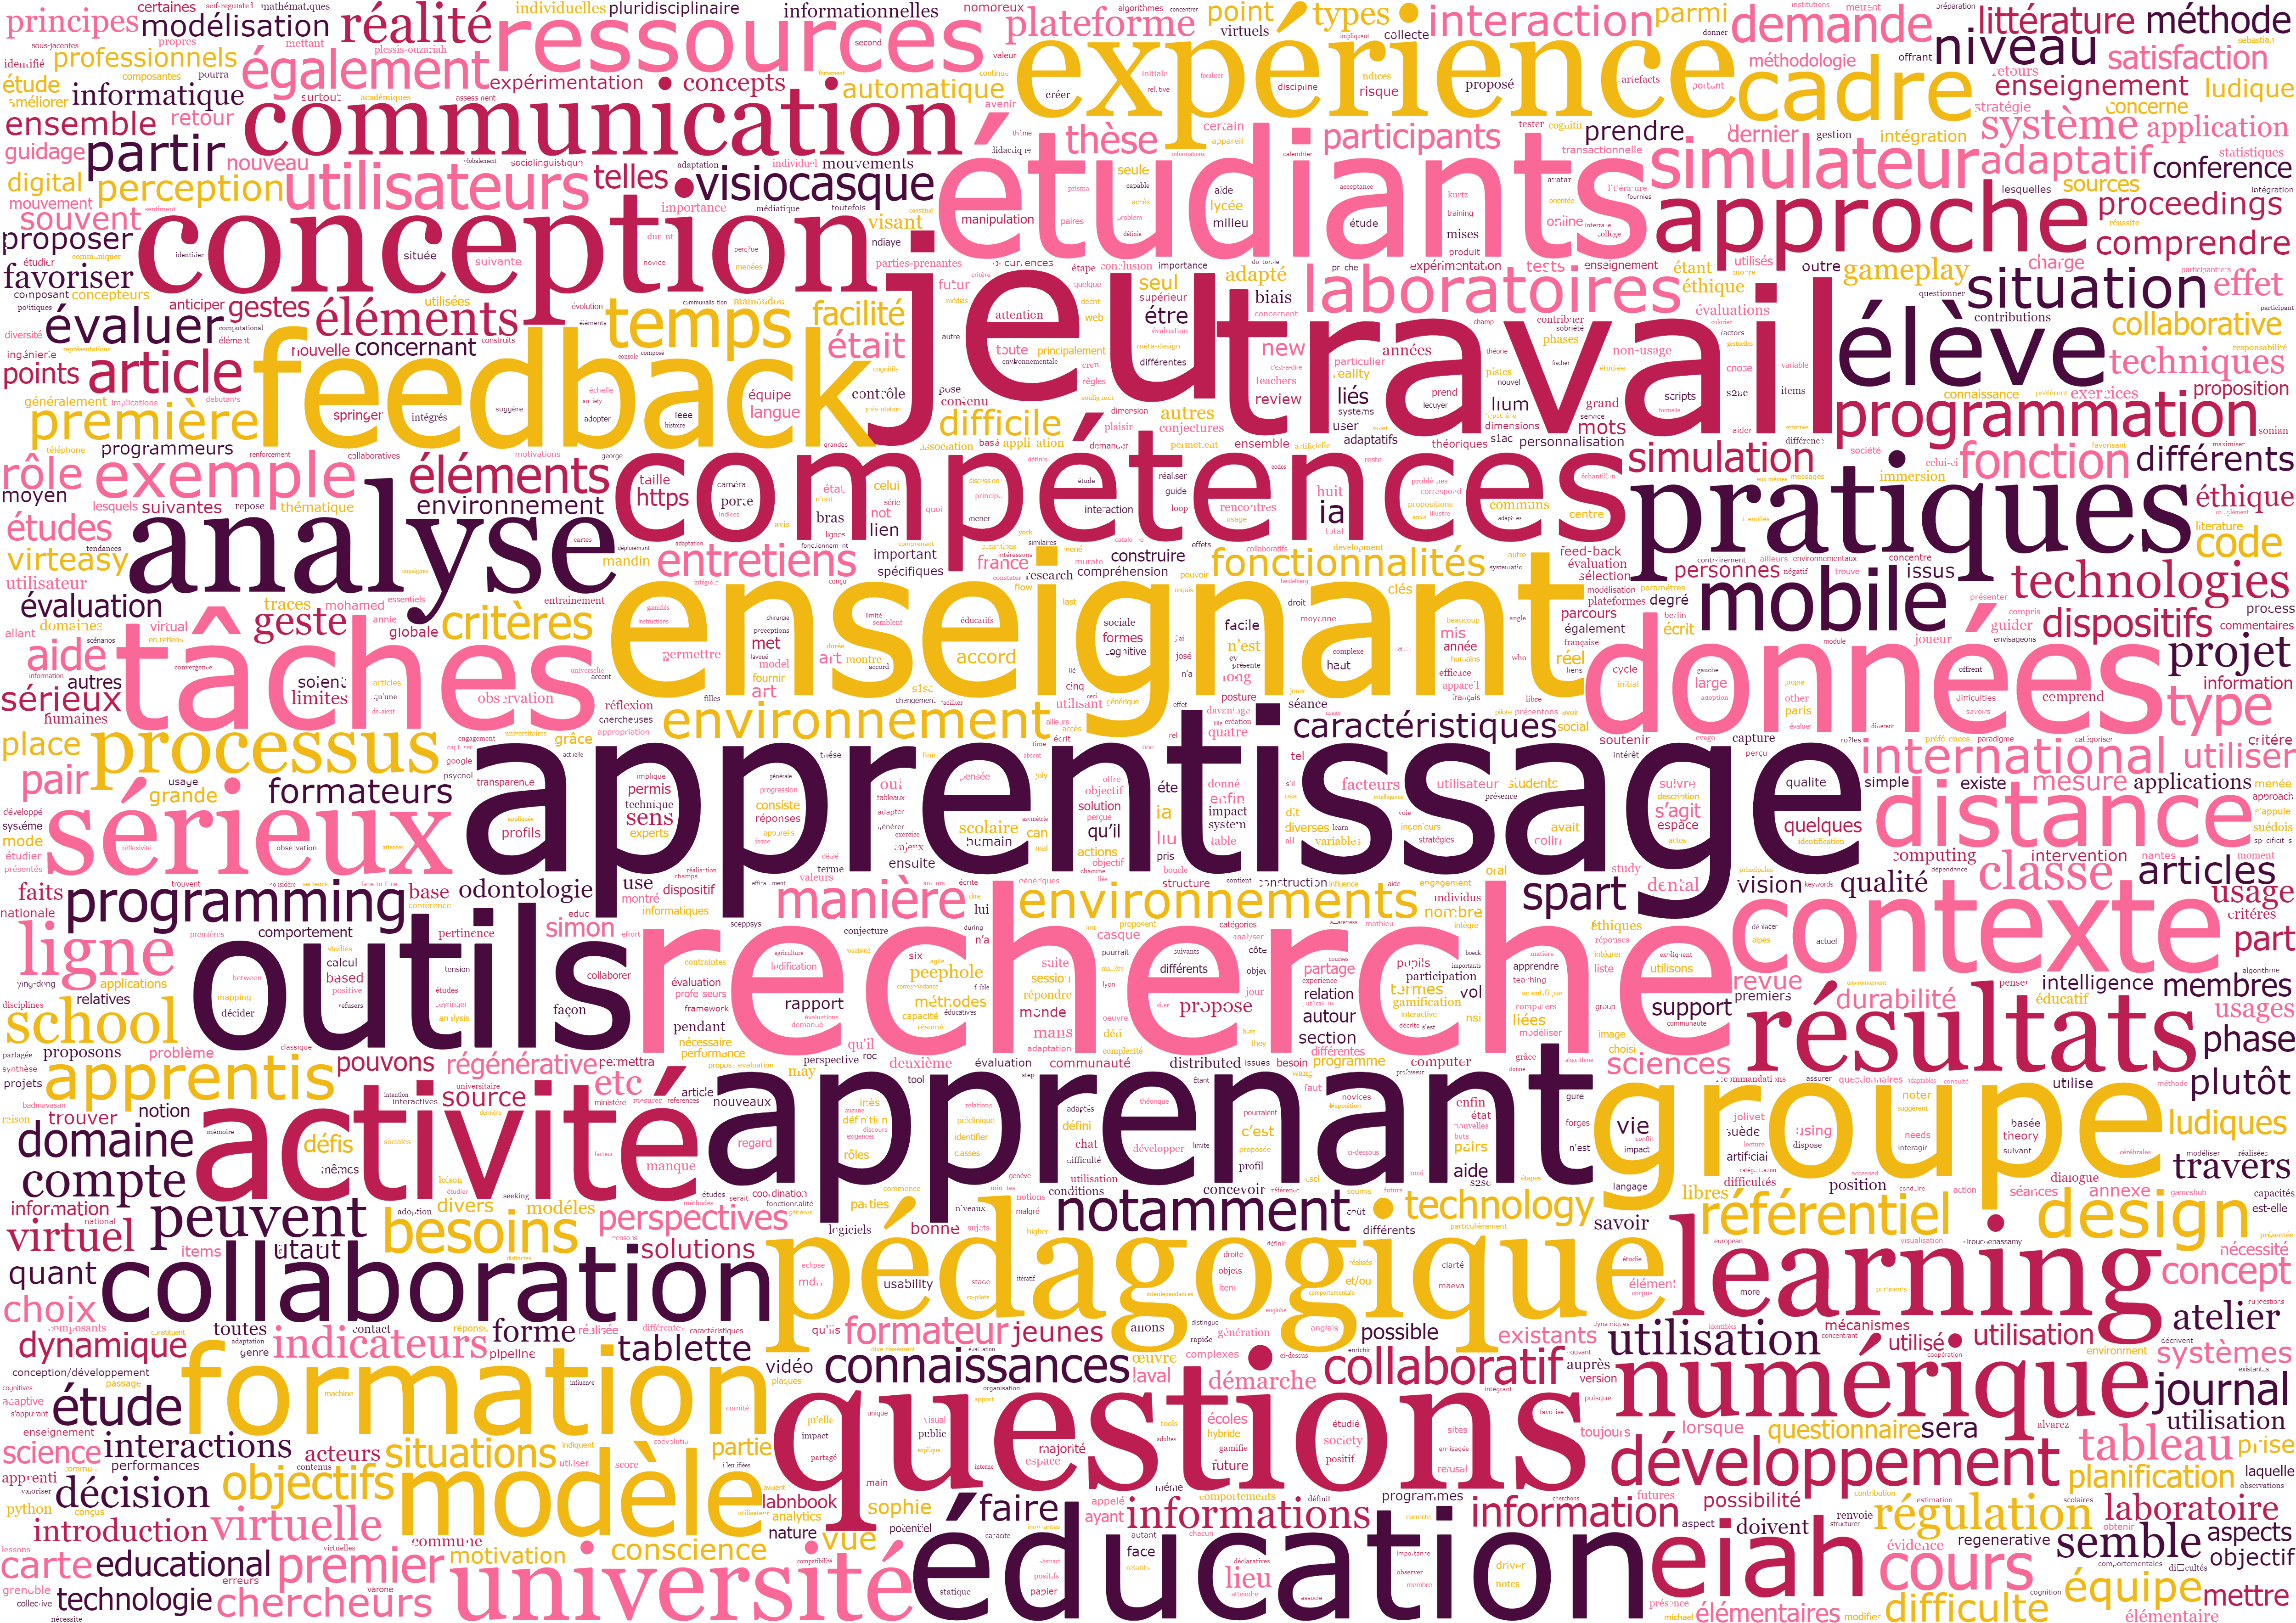
\includegraphics[width=0.7\textwidth]{Content/figures/wordcloud.png}
\end{figure}

\begin{center}
	\begin{Large}
		Édités par Catherine Bonnat et Rémi Venant
	\end{Large}

	\begin{large}
		Les 9 et 10 mai 2022\\
		Université de Lille\\
		France
	\end{large}
\end{center}

\vspace*{\fill}

\begin{figure}[!ht]
	\centering
	\includegraphics[width=.15\textwidth,valign=m]{Content/figures/atief.png}\hfill
	\includegraphics[width=.15\textwidth,valign=m]{Content/figures/cristal.png}\hfill
	\includegraphics[width=.15\textwidth,valign=m]{Content/figures/cirel.png}\hfill
\end{figure}

\noindent Avec le soutien de

\begin{figure}[!ht]
	\centering
	\includegraphics[width=.18\textwidth,valign=m]{Content/figures/regionHautDeFrance.jpg}\hfill
	\includegraphics[width=.18\textwidth,valign=m]{Content/figures/univLille.png}\hfill
	\includegraphics[width=.18\textwidth,valign=m]{Content/figures/interreg.png}\hfill
\end{figure}

\begin{center}
	\small{Les neuvièmes rencontres jeunes chercheur·e·s en EIAH 2022 ont été organisées par l’Université de Lille sous l’égide de l’ATIEF (Association des Technologies de l’Information pour l’Education et la Formation)}
\end{center}

\restoregeometry
\newpage %p1 page de garde
\pageblanche[empty]{} %p2 deuxième de converture

%%%%%%%%%%%%%%%% Table des matière %%%%%%%%%%%%%%%%%%%%%%%%%%%%
\setcounter{secnumdepth}{1}
\setcounter{tocdepth}{2}
\clearpage
\tableofcontents
\newpage %p3, 4, 5

%%%%%%%%%%%%%%%% Comités %%%%%%%%%%%%%%%%%%%%%%%%%%%%
\vspace*{2em} % permet d'aligner verticalement le titre de la section avec celui de la page de droite (puisque logo placé au dessus de l'introduction)
\section{Comités}
\subsection*{Comité de programme}


\subsubsection*{Présidents :}

\begin{itemize}
	\item[] Bonnat Catherine (LIP-TECFA Université de Genève)
	\item[] Venant Rémi (LIUM, Le Mans Université)
\end{itemize}

\subsubsection*{Membres :}

\begin{itemize}
	\item[] Abel Marie-Helene (HEUDIASYC - Univ. de Technologie de Compiègne)
	\item[] Athias Francine (ELLIADD-FR EDUC)
	\item[] Barré Vincent (LIUM, Le Mans Université)
	\item[] Bouchet François (LIP6, Sorbonne Université)
	\item[] Broisin Julien (IRIT, Université Toulouse 3 Paul Sabatier)
	\item[] Brun Armelle (LORIA - Université Nancy 2)
	\item[] Caron Pierre-André (CIREL, Université de Lille)
	\item[] Champagnat Ronan (L3i - Universite de La Rochelle)
	\item[] Champalle Olivier (DICEN ID, Université Paris Est)
	\item[] Crétin-Pirolli Raphaëlle (CREN, Le Mans Université)
	\item[] Desmoulins Cyrille (Université Grenoble Alpes)
	\item[] Dessus Philippe (Univ. Grenoble Alpes, LaRAC)
	\item[] El Mawas Nour (CIREL, Université de Lille)
	\item[] George Sébastien (LIUM, Le Mans Université)
	\item[] Gilliot Jean-Marie (Lab-STICC, IMT Atlantique)
	\item[] Girault Isabelle (LIG, Université de Grenoble Alpes)
	\item[] Grandbastien Monique (LORIA, Universite de Lorraine)
	\item[] Greffier Françoise (ELLIADD, Université de Franche-Comté)
	\item[] Guin Nathalie (LIRIS - Université de Lyon 1)
	\item[] Hamon Ludovic (LIUM - Le Mans Université, France)
	\item[] Iksal Sébastien (LIUM - Le Mans Université, France)
	\item[] Jean-Daubias Stéphanie (LIRIS, Université de Lyon 1)
	\item[] Jolivet Sébastien (LDAR - Université Paris Diderot)
	\item[] Lallé Sébastien (LIP6, Sorbonne Université)
	\item[] Lavoué Elise (LIRIS, Université Jean Moulin Lyon 3)
	\item[] Lebis Alexis (IMT Nord-Europe)
	\item[] Lefevre Marie (LIRIS - Université Lyon 1)
	\item[] Lenne Dominique (HEUDIASYC, Univ. de Technologie de Compiègne)
	\item[] Lourdeaux Domitile (HEUDIASYC, Univ. de Technologie de Compiègne)
	\item[] Luengo Vanda (LIP6, Sorbonne Université)
	\item[] Mandran Nadine (LIG, Université de Grenoble Alpes)
	\item[] Marfisi-Schottman Iza (LIUM, Le Mans Université)
	\item[] Michel Christine (Université de Poitiers)
	\item[] Mohib Najoua (LISEC, Université de Strasbourg)
	\item[] Muratet Mathieu (LIP6, INS HEA)
	\item[] Oubahssi Lahcen (LIUM, Le Mans Université)
	\item[] Perez Sanagustin Mar (IRIT, Université Toulouse 3 Paul Sabatier)
	\item[] Peter Yvan (CRIStAL, Université de Lille)
	\item[] Piau-Toffolon Claudine (LIUM, Le Mans Université)
	\item[] Pirolli Fabrice (CREN, Le Mans Université)
	\item[] Poirier Franck (Lab-STICC, IMT Atlantique)
	\item[] Rebai Issam (IMT Atlantique)
	\item[] Reffay Christophe (ELLIADD \& ESPE, Université de Franche-Comté)
	\item[] Reyssier Stéphanie (ECP - Université Lumière Lyon 2)
	\item[] Rosselle Marilyne (MIS, Université de Picardie)
	\item[] Sanchez Eric (Université Fribourg)
	\item[] Secq Yann (CRIStAL, Université de Lille)
	\item[] Sehaba Karim (LIRIS - Université Lumière Lyon 2)
	\item[] Silvestre Franck (IRIT, IUT de Rodez)
	\item[] Trgalova Jana (S2HEP, Université Lyon 1)
	\item[] Vadcard Lucile (LARAC, Université Grenoble Alpes)
	\item[] Vermeulen Mathieu (IMT Nord-Europe)
	\item[] Yessad Amel (LIP6, Sorbonne Université)
\end{itemize}

\subsection*{Coordinateurs des ateliers et symposia : }

\begin{itemize}
	\item[] Reyssier Stéphanie (LIRIS - Université Lumière Lyon 2)
	\item[] Lebis Alexis (IMT Nord Europe)
\end{itemize}

\subsection*{Comité d'organisation :}

\begin{itemize}
	\item[] Caron Pierre-André (CIREL, Université de Lille)
	\item[] El Mawas Nour (CIREL, Université de Lille)
	\item[] Léonard Marielle (CIREL \& CRIStA, Université de Lille)
	\item[] Peter Yvan (CRIStAL, Université de Lille)
	\item[] Secq Yann (CRIStAL, Université de Lille)
\end{itemize}
\newpage %p 6, 7

%%%%%%%%%%%%%%%% Introduction %%%%%%%%%%%%%%%%%%%%%%%%%%%%
\logoConf % replace le logo de la conf au dessus du titre de la section
\section{Introduction aux actes}
Les dixièmes Rencontres Jeunes Chercheuses et Chercheurs en EIAH (RJC EIAH 2024) se sont tenues à Laval du 4 au 7 juin 2024. Ces rencontres sont une occasion particulièrement importante pour les jeunes chercheuses et chercheurs de la communauté EIAH (Environnements Informatiques pour l’Apprentissage Humain) de pouvoir se rencontrer et échanger avec des chercheuses et chercheurs autour de leurs travaux. 

En effet, les RJC EIAH, organisées tous les 2 ans sous l’égide de l’ATIEF (Association des Technologies de l'Information pour l'Éducation et la Formation) visent le développement de la communauté EIAH par la formation des doctorantes et doctorants issus des différentes disciplines inhérentes au domaine des EIAH et la diffusion de leurs travaux. 

\begin{figure}[!h]
	\centering
	\includegraphics[width=0.7\textwidth]{Content/figures/carteComplete.png}
	\caption{Répartition géographique des publications des RJC EIAH 2024}
	\label{f:repGeoPubli}
\end{figure}

L’édition 2024 a retenu l’attention de 24 jeunes chercheuses et chercheurs qui ont soumis une contribution sous forme d’articles longs de 12 pages pour 17 d’entre eux, et d'articles courts de 4 pages pour 7 autres. 
Chacune des communications ont été évaluées par 2 membres du comité de programme issus pour l'un des sciences humaines et sociales (SHS) et pour l'autre de l'informatique. À l’issue de cette phase d'évaluation, 14 propositions ont été acceptées sous la forme d’articles longs, et 9 ont été acceptées sous la forme d’articles courts. Nous remercions d'ailleurs le comité de programme pour la qualité  des relectures et les commentaires conséquents et pédagogiques qui permettent l’amélioration des articles proposés et des présentations lors de la conférence.

Les articles longs acceptés ont été présentés lors de la conférence sous la forme d'une présentation orale et les articles courts à travers une présentation de poster.

Les contributions proviennent essentiellement d’universités françaises, mais comptent également des travaux issus de Suisse (2) (voir Figure \ref{f:repGeoPubli}). Les publications proviennent ainsi de 15 laboratoires de recherches différents.

\begin{figure}[!h]
	\centering
	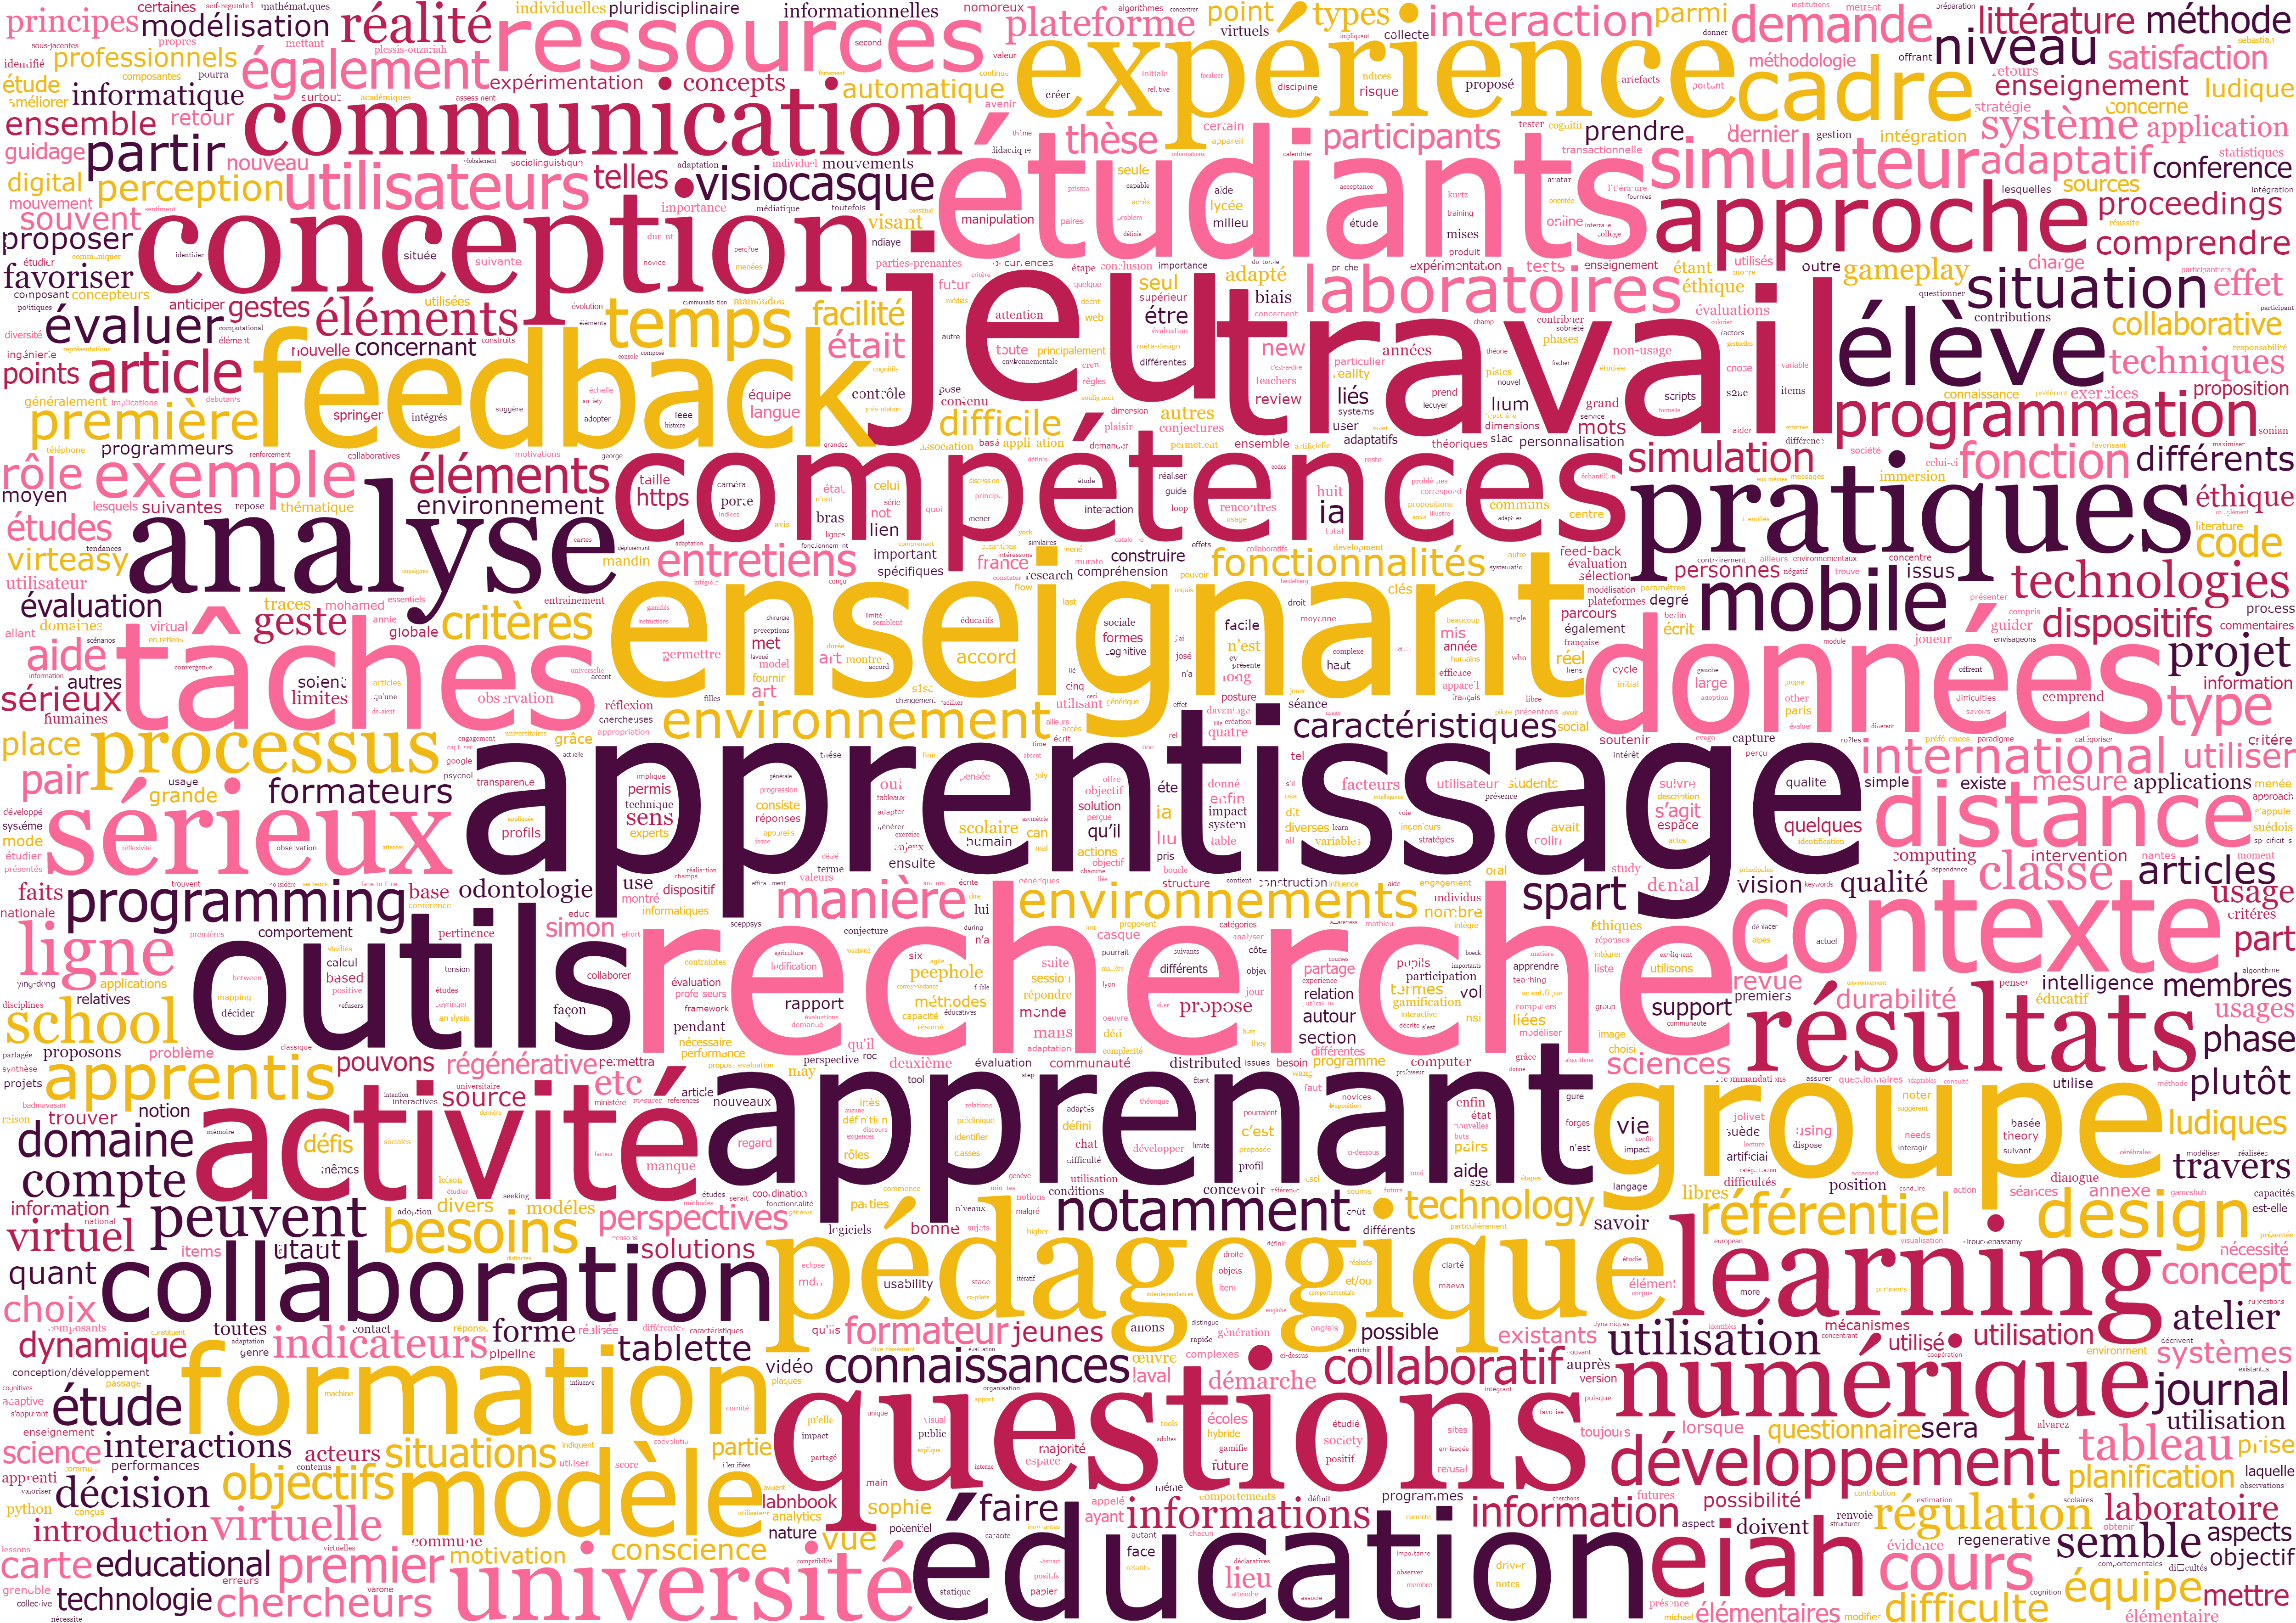
\includegraphics[width=0.7\textwidth]{Content/figures/wordcloud.png}
	\caption{Nuage de mots des contributions à RJC-EIAH 2022}
	\label{f:wordCloud}
\end{figure}

Les contributions se répartissent entre les disciplines de l’informatique (14) et des sciences humaines et sociales (8). Pour cette édition, 2 grandes thématiques transversales aux disciplines ont été abordées par un grand nombre des travaux présentés~: près des trois quarts des contributions portent sur les formes d'apprentissage incluant majoritairement les jeux sérieux, la réalité virtuelle/augmentée/mixte et la simulation~; les travaux sur les usages sont également à l'honneur avec près de trois cinquièmes des articles, certains abordent la question sur l'axe des \textit{learning analytics} alors que d'autre sont orientés sur les modalités d'intégration et les méthodes d'évaluation. La figure \ref{f:wordCloud} qui expose les termes les plus présents dans les contributions fait état de ces tendances.

Ces contributions ont donc fait l’objet de quatre sessions distinctes : 
\begin{enumerate}
	\item Analyse d'usage(s) et de pratiques ;
	\item Méthodes d'évaluation des dispositifs d'apprentissage / de formation dans les EIAH ;
	\item Méthodes de conception des EIAH et Systèmes adaptatifs et personnalisation de l'apprentissage ;
	\item Modalités d'organisation communautaires (collaboration, coopération...).
\end{enumerate}

Ces rencontres jeunes chercheur.e.s ont également accueilli une conférence de la Professeur ... de l'Université ..., qui porte sur ... ; aussi nous la remercions chaleureusement.

Nous remercions aussi l’ATIEF, les différents membres des comités de programme, d'organisation et de coordination des ateliers ainsi que les différents partenaires pour leur soutien à cette manifestation et plus particulièrement l’Université du Mans qui a accueilli les rencontres sur son site de Laval.

Pour finir, nous remercions chaleureusement tous les chercheurs en EIAH, et en particulier les jeunes chercheuses et chercheurs sans qui ces rencontres n’auraient pas lieu.

\vspace*{2em}
\begin{flushright}
	Sonia Mandin et Mathieu Muratet, co-présidents du comité de programme
\end{flushright}
\newpage %p8, 9, 10

%%%%%%%%%%%%%%%% Conférenciés invités %%%%%%%%%%%%%%%%%%%%%%%%%%%%
\vspace*{2em}
\section{Conférencière invitée}
\begin{center}
	\noindent\large\textbf{ Personnaliser l’Apprentissage dans l’Enseignement Supérieur ?\\
		Pas si simple. }
\end{center}

\begin{center}
	\begin{tabular}{@{}c@{}}
		Agathe Merceron, Professeure d'Informatique\\
		Computer Science at the Berlin University of Applied Sciences, Germany\\
		\email{merceron@bht-berlin.de}
	\end{tabular}
\end{center}

\subsection*{Résumé}
Dans l’apprentissage comme dans les autres domaines, nous avons de plus en plus de données numériques que nous pouvons donc analyser avec des algorithmes. 
Et nous faisons des découvertes intéressantes ! 
Par exemple, nous pouvons prédire si un étudiant ou une étudiante va interrompre ses études avec une exactitude de plus de 90\% dans certains cas.
Ou bien encore, nous pouvons extraire des comportements d’étudiants dans les plateformes numériques et relier certains comportements avec un plus grand succès académique. 
Comment utiliser ces ``trouvailles'' pour aider les étudiants à mieux étudier ? 
Que pensent les étudiants de ces “trouvailles” et que souhaitent-ils, que souhaitent-elles ? 
Dans cette conférence, je vais présenter quelques ``trouvailles'' que nous avons faites dans nos projets et comment nous essayons d’impliquer les étudiants pour recueillir leurs opinions et points de vue. 

\subsection*{Biographie}

\begin{wrapfigure}[12]{R}{0.25\textwidth}
	\centering\includegraphics[width=0.24\textwidth]{Content/figures/AgatheMerceron}
\end{wrapfigure}
\textbf{Agathe Merceron} est Professeure émérite d’Informatique à l’Université des
Sciences Appliquée de Berlin où  elle y a dispensé différents enseignements
tels que l’introduction à la programmation, les fondements théoriques de
l’Informatique ou l’apprentissage machine. 
Jusqu'à Mars 2022, elle était directrice des programmes d'enseignement en ligne d'Informatique et des  médias pour les Bachelors et Masters. 
Sa recherche porte actuellement sur les Environnements Informatiques pour l'Apprentissage Humain avec une attention sur la fouille de données d'apprentissage (\textit{Education Data Mining}) et sur les \textit{Learning Analytics}. 
Elle est impliquée nationalement et à l'international dans ces domaines, a été la président de comités de programme de conférences et workshops, en particulier pour les conférences internationales ``Educational Data Mining'' (EDM) et ``Learning Analytics and Knowledge'' (LAK), est éditrice de la revue  ``Journal of Educational Data Mining'' (JEDM) et est membre du comité de programme du journal ''Sciences et Technologies de l'Information et de la  Communication pour l'Éducation et la Formation'' (STICEF).






\newpage %p11

% Fin sur page impair : il faut absolument finir ici sur une page impaire. Retirez la page blanche suivante au besoin.
\pageblanche %p12

%%%%%%%%%%%%%%%% SESSION D'ARTICLES 1 %%%%%%%%%%%%%%%%%%%%%%%%%%%%
%Vérifier que l'on commence bien sur une page impaire, pour que le premier article débute sur une page paire

% les pages de titre doivent toujours être sur une page impaire
% tous les articles sauf le dernier doivent avoir un nombre de pages pair (on ajoute une page blanche sinon)
% Le  dernier article de la session doit avoir sur un nombre de pages impair  (on ajoute une page blanche sinio) pour que la page de titre de session soit sur une page impair

\pageTitreSession[Animateur de session : Sébastien Jolivet]{Session de communications 1 : Conception pour les jeux sérieux} %p13

%ART 10: 8 pages
\includepdf[pages={-}, pagecommand={\markboth{Estelle Prior}{Partage des savoirs dans une réunion de co-conception de jeux épistémiques numériques...}}, fitpaper=false,addtotoc={1, subsection, 2, Partage des savoirs dans une réunion de co-conception de jeux épistémiques numériques en recherche orientée par la conception \newline \protect\textit{Estelle Prior}, ART10}]{VendorPDF/10.pdf}


%ART 15: 8 page, dernier article de session : nécessite \pageblanche
\includepdf[pages={-}, pagecommand={\markboth{Enzo Simonnet}{Projet Lex$:$gaMe : des mots et des motivés}}, fitpaper=false, addtotoc={1, subsection, 2, Projet Lex$:$gaMe : des mots et des motivés \newline  \protect\textit{Enzo Simonnet}, ART15}]{VendorPDF/15.pdf}
\pageblanche

%%%%%%%%%%%%%%%% SESSION D'ARTICLES 2 %%%%%%%%%%%%%%%%%%%%%%%%%%%%
\pageTitreSession[Animatrice de session : Catherine Bonnat]{Session de communications 2 : Analytiques pour l’apprenant et l’enseignant}

% ART 03: 7 pages, pas en fin de session : nécessite \pageblanche
\includepdf[pages={-}, pagecommand={\markboth{Mélina Verger}{Investiguer la notion d’équité algorithmique dans les environnements informatiques...}}, fitpaper=false, addtotoc={1, subsection, 2, Investiguer la notion d’équité algorithmique dans les environnements informatiques pour l’apprentissage humain \newline  \protect\textit{Mélina Verger}, ART03}]{VendorPDF/03.pdf}
\pageblanche % Article 3 à un nombre de page impair

%ART 21: 8 pages
\includepdf[pages={-}, pagecommand={\markboth{Esther Félix}{Introduction à l'explicabilité dans les feedback automatisés fournis aux apprenants}}, fitpaper=false, addtotoc={1, subsection, 2, Introduction à l'explicabilité dans les feedback automatisés fournis aux apprenants \newline  \protect\textit{Esther Félix}, ART21}]{VendorPDF/21.pdf}

%ART 18: 7 pages, dernier article de session : pas besoin de \pageblanche
\includepdf[pages={-}, pagecommand={\markboth{Ibtissem Bennacer}{iTeachApp, un outil d'auto-évaluation et de soutien pour les enseignants}}, fitpaper=false, addtotoc={1, subsection, 2, iTeachApp\, un outil d'auto-évaluation et de soutien pour les enseignants \newline  \protect\textit{Ibtissem Bennacer}, ART18}]{VendorPDF/18.pdf}


%%%%%%%%%%%%%%%% SESSION DE POSTER %%%%%%%%%%%%%%%%%%%%%%%%%%%%
\pageTitreSession{Session de posters}

%ART 31: 4 pages
\includepdf[pages={-}, pagecommand={\markboth{Esteban Villalobos}{Mesurer l'autorégulation dans des contextes d'apprentissage mixtes}}, fitpaper=false, addtotoc={1, subsection, 2, Mesurer l'autorégulation dans des contextes d'apprentissage mixtes \newline  \protect\textit{Esteban Villalobos}, ART31}]{VendorPDF/31.pdf}

%ART 02: 5 pages, dernier article de session : pas besoin de \pageblanche
\includepdf[pages={-}, pagecommand={\markboth{Myriam Leclaire}{Jeux de rôles et autoconfrontations collectives comme outils pédagogiques...}}, fitpaper=false, addtotoc={1, subsection, 2, Jeux de rôles et autoconfrontations collectives comme outils pédagogiques de développement des compétences collaboratives interprofessionnelles des étudiants en santé \newline  \protect\textit{Myriam Leclaire}, ART02}]{VendorPDF/02.pdf}


% dernière session terminée, retour aux en-têtes généraux
\resetHeadings

%%%%%%%%%%%%%%%%Symposia%%%%%%%%%%%%%%%%%%%%%%%%%%%%
\pageTitreSession{Ateliers et Symposia}

\vspace*{2em}
\begin{center}
	\subsection{Symposium 1 : Conception et évaluation de tableaux de bord d’apprentissage}
\end{center}


\vspace{1em}
\begin{center}
	\begin{tabular}{@{}c@{}}
		Sébastien Iksal\textsuperscript{1}, Madjid Sadallah\textsuperscript{2}, Katia Quelennec\textsuperscript{3}\\
		\textsuperscript{1}LIUM, Le Mans Université\\
		\textsuperscript{2}Lab-STICC, IMT Atlantique\\
		\textsuperscript{3}Université de Lille
	\end{tabular}
\end{center}

\vspace{2em}

Le domaine des Learning Analytics offre de nouvelles perspectives d’analyse des différents processus d’apprentissage. Dans cet atelier, nous poursuivons les travaux sur le développement d’outils permettant l’appropriation des Learning Analytics par les utilisateurs potentiels et la capture des besoins utilisateurs.

L’atelier Quels tableaux de bord pour les acteurs de l’éducation ? organisé dans le cadre de la conférence EIAH2017 a permis d’identifier les différentes dimensions et les enjeux liés aux tableaux de bord d’apprentissage. Depuis, un outil de conception participative a été proposé et utilisé dans des séances de travail par différentes équipes de la communauté, démontrant l’intérêt pour ce type de démarches.

Dans le cadre de la conférence EIAH 2021, un deuxième atelier Conception participative de tableaux de bord d’apprentissage a été réalisé avec l’objectif d’identifier les usages potentiels de tels outils et de dégager des propositions pour développer de nouveaux outils à disposition de la communauté. Suite à cela une nouvelle version de l’outil de conception participative PaDLAD V2 a été proposé et utilisé. Dans le cadre de cet atelier, nous souhaitons avancer sur la capitalisation de ce qui a été mené dans les différentes expériences de conception et de réfléchir à l’évaluation, l’adaptation et le processus qualité lié aux tableaux de bord d’apprentissage. L’objectif final étant la création du groupe de travail ATIEF sur le sujet.

\newpage

\vspace*{2em}
\begin{center}
	\subsection{Symposium 2 : Cadres théoriques, état de l’art pour les EIAH ?}
\end{center}

\vspace{1em}
\begin{center}
	\begin{tabular}{@{}c@{}}
		Nadine Mandran\textsuperscript{1}, Nour El Mawas\textsuperscript{2}\\
		\textsuperscript{1}LIG, Université de Grenoble Alpes \\
		\textsuperscript{2}CIREL, Université de Lille
	\end{tabular}
\end{center}

\vspace{2em}

Les notions de cadres théoriques, d’état de l’art scientifique, de positionnement, de travaux connexes, de modèles d’analyses sont des outils pour construire d’une part une problématique et identifier des manques auxquels la recherche peut apporter des contributions. Ces différentes dimensions sont importantes dans toutes disciplines. Cependant dans le cadre d’un travail au cœur de plusieurs disciplines, le sens et la finalité de ces concepts ne sont pas toujours partagés. Cette méconnaissance entraîne parfois des difficultés pour co-élaborer des projets de recherche. De plus, la confusion entre ces termes met parfois en difficulté les doctorant.e.s.

L’objectif de l’atelier est d’échanger autour de ces concepts selon les disciplines présentes dans les EIAH,  de mieux se comprendre sur ces concepts, d’échanger sur les méthodes de mobilisation de la littérature et de construction de l’état de l’art.

Des activités seront organisées pour que les doctorant.e.s et les chercheurs seniors confrontent leurs points de vue et leurs méthodes.

\newpage

\vspace*{2em}
\begin{center}
	\subsection{Symposium 3 : La notion de compétence pour les EIAH}
\end{center}

\vspace{1em}
\begin{center}
	\begin{tabular}{@{}c@{}}
		Mathieu Vermeulen\textsuperscript{1}, Nathalie Guin\textsuperscript{2}\\
		\textsuperscript{1}IMT Nord-Europe\\
		\textsuperscript{2}LIRIS, Université de Lyon 1
	\end{tabular}
\end{center}

\vspace{2em}

La notion de compétence est devenue centrale dans nombre de situations liées à la formation et à l’apprentissage, que ce soit en formation initiale, continue ou professionnelle. L’intégration de l’approche par compétences dans les cycles primaires et secondaires est aujourd’hui effective et sa mise en place est en cours dans le supérieur. Outre le besoin d’information et de formation à ce nouveau paradigme, le mot compétence en tant que tel engendre des incompréhensions d’ordre sémantique ou fonctionnelles.  Le caractère protéiforme de cette notion rend son appropriation difficile, en particulier parce qu’elle est liée au contexte de son utilisation.

En ce qui concerne les EIAH, la multiplicité des définitions et le croisement des nombreuses expertises, ainsi que la diversité des cadres épistémologiques de la recherche en EIAH, impactent les travaux menés par les chercheurs du domaine, conduisant à un certain flou autour de la notion de compétence. Pour autant, de récents projets (ANR xCALE, ANR COMPER, iSite ULNE APACHES, etc.) travaillent sur son intégration dans les artefacts informatiques avec des objectifs variés : la modélisation des compétences, l’assistance à l’évaluation de celles-ci, la personnalisation des parcours des apprenants, l’accompagnement à la mise en place des approches par compétences, etc. De fait, le besoin d’offrir un cadre favorisant une meilleure appropriation du concept de compétence, et donc une intégration efficiente dans les travaux de recherche en EIAH, semble aujourd’hui devenir indispensable.

Cet atelier fait suite au Séminaire APACHES d’octobre 2021 et propose, au travers de présentations et d’activités participatives, de travailler sur cette notion de compétence, sur son intégration aux EIAH et en particulier sur la co-élaboration d’une grille de questions permettant aux chercheurs de positionner la compétence dans leurs travaux en fonction de leurs objectifs et de leurs contextes.

\newpage

\vspace*{2em}
\begin{center}
	\subsection{Symposium 4 : Adaptation et génération dans les EIAH}
\end{center}

\vspace{1em}
\begin{center}
	\begin{tabular}{@{}c@{}}
		Pierre Laforcade\textsuperscript{1}, Sébastien Jolivet\textsuperscript{2}, Marie Lefevre\textsuperscript{3}\\
		\textsuperscript{1}LIUM, Le Mans Université\\
		\textsuperscript{2}LDAR, Université Paris Diderot\\
		\textsuperscript{3}LIRIS, Université Lyon 1
	\end{tabular}
\end{center}

\vspace{2em}

L’adaptation dans un EIAH est une activité complexe, pluri-disciplinaire, qui nécessite d’être appréhendée en prenant en compte ses nombreuses dimensions (didactique, pédagogique, ludique, motivationnelle, informatique...), ses perspectives (cibles, sources et objectifs de l’adaptation), ainsi que les différents acteurs concernés.

L’atelier proposé dans le cadre de RJC’22 s’intéresse plus particulièrement aux dimensions ludiques et motivationnelles. L’atelier est organisé sous la forme d’un symposium autour de 4 invités :

\begin{itemize}
	\item Élise Lavoué (LIRIS), chercheure reconnue pour ses travaux sur les thématiques de l’adaptation et de la ludification en EIAH ; elle présentera ces derniers travaux autour de la gamification adaptative et l’engagement des apprenants.
	\item Bertrand Marne (ICAR), chercheur reconnu pour ses travaux en ingénierie des jeux sérieux ;
	\item Bérénice Lemoine (LIUM), doctorante abordant la génération d’activités d’apprentissage ludiques adaptées dans un jeu sérieux ;
	\item Luca Pelissero-Witoslawski (HEUDIASYC), doctorant abordant la génération dynamique de situations stressantes en environnement virtuel d’apprentissage.
\end{itemize}
% selin le nombre de page ici, il peut être nécessaire de place une  \pageblanche

%%%%%%%%%%%%%%%%Partenaires%%%%%%%%%%%%%%%%%%%%%%%%%%%%
\newpage
\vspace*{2em}
\section{Partenaires}
\iffalse
\begin{figure}[!ht]
	\centering
	\footnotesize
	\stackunder[5pt]{\includegraphics[width=0.4\textwidt,valign=m]{Content/figures/atief.png}}{Association des Technologies de l'Information pour l'Education et la Formation}
	\hfill
	\stackunder[5pt]{\includegraphics[width=0.4\textwidt,valign=m]{Content/figures/univLille.png}}{Université de Lille}
	
	\iffalse
	\vspace{0.08\textheight}
	
	\stackunder[5pt]{\includegraphics[width=0.4\textwidt,valign=m]{Content/figures/regionHautDeFrance.jpg}}{Région Haut de France}
	\hfill
	\stackunder[5pt]{\includegraphics[width=0.4\textwidt,valign=m]{Content/figures/interreg.png}}{Interreg France-Wallonnie-Vlaanderen - Teach Transition}
	
	\vspace{0.08\textheight}
	
	\stackunder[5pt]{\includegraphics[width=0.4\textwidt,valign=m]{Content/figures/cirel.png}}{Centre Interuniversitaire de Recherche en Éducation de Lille}
	\hfill
	\stackunder[5pt]{\includegraphics[width=0.4\textwidt,valign=m]{Content/figures/cristal.png}}{Centre de Recherche en Informatique, Signal et Automatique de Lille}
	\fi
\end{figure}
\fi

\begin{figure}[!ht]
	\begin{subfigure}{0.4\textwidth}
		\includegraphics[width=\textwidth]{Content/figures/atief.png}
		\caption{Association des Technologies de l'Information pour l'Education et la Formation}
	\end{subfigure}
	\hfill
	\begin{subfigure}{0.4\textwidth}
		\includegraphics[width=\textwidth]{Content/figures/univLille.png}
		\caption{Université de Lille}
	\end{subfigure}

	\vspace{0.08\textheight}
	
	\begin{subfigure}{0.4\textwidth}
		\includegraphics[width=\textwidth]{Content/figures/regionHautDeFrance.jpg}
		\caption{Région Haut de France}
	\end{subfigure}
	\hfill
	\begin{subfigure}{0.4\textwidth}
		\includegraphics[width=\textwidth]{Content/figures/interreg.png}
		\caption{Interreg France-Wallonnie-Vlaanderen - Teach Transition}
	\end{subfigure}
	
	\vspace{0.08\textheight}
	
	\begin{subfigure}{0.4\textwidth}
		\includegraphics[width=\textwidth]{Content/figures/cirel.png}
		\caption{Centre Interuniversitaire de Recherche en Éducation de Lille}
	\end{subfigure}
	\hfill
	\begin{subfigure}{0.4\textwidth}
		\includegraphics[width=\textwidth]{Content/figures/cristal.png}
		\caption{Centre de Recherche en Informatique, Signal et Automatique de Lille}
	\end{subfigure}
\end{figure}

\pageblanche % pour finir sur 2 pages 

%4ème de couverture
\thispagestyle{empty}
%\newgeometry{left=3cm,bottom=0.1cm}
\newgeometry{bottom=1cm,top=1cm}

\hspace{0pt}
\vfill

\logoConf[0.7]
\begin{center}
	\Huge{Actes des neuvièmes rencontres jeunes chercheur·e·s en EIAH}
	
	\vspace{0.7em}
	
	\Large{\textit{Environnements Informatiques pour l'Apprentissage Humain}}
	
	\vspace{0.7em}
	
	\begin{Large}
		Édités par Catherine Bonnat et Rémi Venant
	\end{Large}
	
	\begin{large}
		Les 9 et 10 mai 2022\\
		Université de Lille\\
		France
	\end{large}
\end{center}

\vfill
\hspace{0pt}

\restoregeometry

\end{document}
